\begin{figure}[ht!]
    \centering
    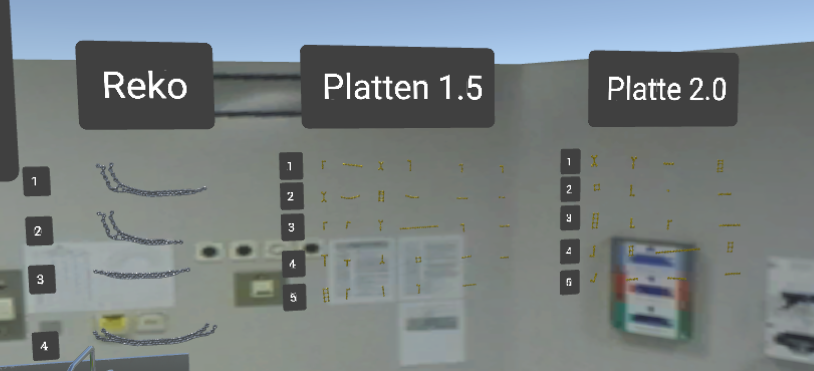
\includegraphics[width=\linewidth]{images/implementation/features/procedures/metal_plates_1.png}
    \caption{\label{fig::FeatureMetalPlate} Osteosynthesis Plates Overview}
\end{figure}

The osteosynthesis plates procedure consists of two steps before adding it as a step to the project case.
First, users have to chose which plate to use (Figure \ref{fig::FeatureMetalPlate}).
The user can chose from four reconstruction plates, 29 1.5mm plates and 20 2.0mm plates.
The optimal plates to use vary due to the pathology of the patient and the previously performed procedures.
After selecting the proper plate, a number of indicators will show to the user (Figure \ref{fig::FeatureMetalPlate2}).
In the context of the osteosynthesis plates, these indicators are "control points", with which the user can bend and twist the plates.
Bending and twisting is performed by chosing a control point via hovering them with the users free hand and grabbing them.
Then, the user has to translate and rotate the control point in the desired manner.
\begin{figure}
  \centering
  \begin{minipage}{.5\textwidth}
    \centering
    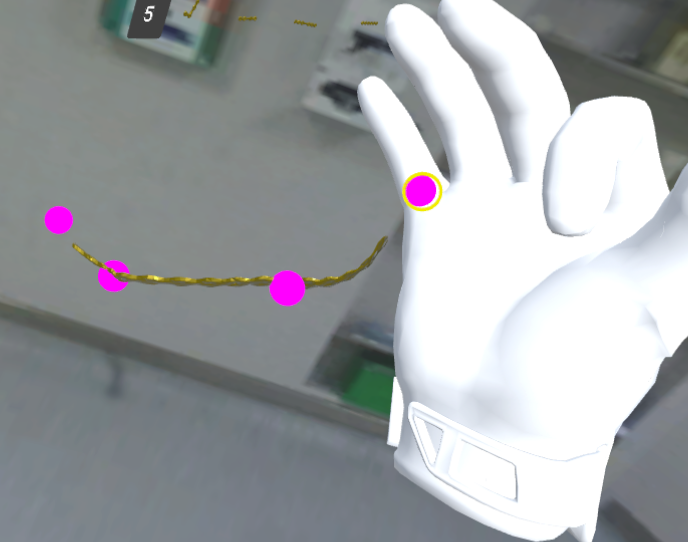
\includegraphics[width=0.95\linewidth]{images/implementation/features/procedures/metal_plates_2.png}
  \end{minipage}%
  \begin{minipage}{.5\textwidth}
    \centering
    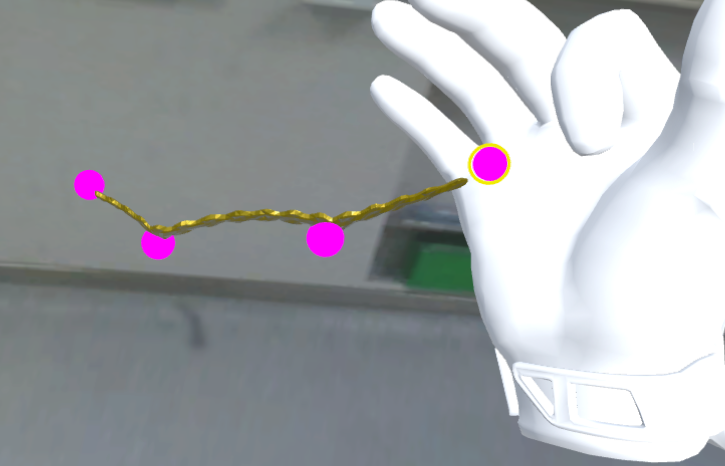
\includegraphics[width=0.95\linewidth]{images/implementation/features/procedures/metal_plates_3.png}
  \end{minipage}
  \caption{\label{fig::FeatureMetalPlate2}Osteosynthesis Plates Modifications. User can translate and rotate "control points" to perform modifications to the plates shape} 
\end{figure}

The user can then observe in which way this has affected the shape of the metal plate and either position the plate on the patient or perform more modifications to the plates via controlpoints.
The correct modification of the metal plates differs quite a lot from real life modifications to the plates.
However even though there is a slight learning curve to it, the modification is consistent and predictable (Figure \ref{fig::FeatureMetalPlate2}).

